\documentclass[a4paper,12pt]{extarticle}

\usepackage[utf8]{inputenc}
\usepackage[margin=0.9in]{geometry}
\usepackage{graphicx}
\usepackage{tikz}
\usetikzlibrary{shapes.callouts,decorations.pathreplacing,calligraphy}
\usepackage{igo}
\usepackage{soul}

\setlength{\fboxrule}{2pt}
\newcommand{\rectangle}{\fboxsep25pt\fbox{\rule{0pt}{0pt}\rule{0pt}{10pt}}}
\newcommand{\smallrectangle}{\fboxsep10pt\fbox{\rule{10pt}{0pt}\rule{0pt}{10pt}}\hspace{5pt}}

\newcommand{\problem}[7]{
\begin{center}
  #1

  \bigskip
  
\cleargoban  
\white{#2}
\black{#3}
\largegoban
\gobansize{9}
\showgoban[a1,i9]

\bigskip

#4
\end{center}

\ifnum#5=0
\begin{tikzpicture}[remember picture, overlay]
  \draw (0,5) node (penguin) {\includegraphics[width=2cm]{#6}};
  \draw (1.5,7) node[ellipse callout,draw,font=\Large,callout absolute pointer={(0.4,6)}] {#7};
\end{tikzpicture}
\else
\begin{tikzpicture}[remember picture, overlay]
  \draw (15,5) node (penguin) {\includegraphics[width=2cm]{#6}};
  \draw (13.5,7) node[ellipse callout,draw,font=\Large,callout absolute pointer={(14.6,6)}] {#7};
\end{tikzpicture}
\fi
\begin{tikzpicture}[remember picture, overlay]
  \draw (4.3,3.1) node[font=\small] {a};
  \draw (5.05,3.1) node[font=\small] {b};
  \draw (5.8,3.1) node[font=\small] {c};
  \draw (6.55,3.1) node[font=\small] {d};
  \draw (7.3,3.1) node[font=\small] {e};
  \draw (8.05,3.1) node[font=\small] {f};
  \draw (8.8,3.1) node[font=\small] {g};
  \draw (9.6,3.1) node[font=\small] {h};
  \draw (10.35,3.1) node[font=\small] {j};
  %\draw (11.05,3.1) node[font=\small] {l};

  \draw (3.5,3.6) node[font=\small] {1};
  \draw (3.5,4.4) node[font=\small] {2};
  \draw (3.5,4.4 + 0.775) node[font=\small] {3};
  \draw (3.5,4.4 + 2*0.775) node[font=\small] {4};
  \draw (3.5,4.4 + 3*0.775) node[font=\small] {5};
  \draw (3.5,4.4 + 4*0.775) node[font=\small] {6};
  \draw (3.5,4.4 + 5*0.775) node[font=\small] {7};
  \draw (3.5,4.4 + 6*0.775) node[font=\small] {8};
  \draw (3.5,4.4 + 7*0.775) node[font=\small] {9};    
\end{tikzpicture}
}

\begin{document}
\Huge

\begin{center}
  Draw stone to play.

  \vspace{2cm}

  \cleargoban  
  \white{f5}
  \black{f4,g5,e5}
  \largegoban
  \gobansize{9}
  \showgoban[a1,i9]

  \begin{tikzpicture}[remember picture, overlay]
    \draw (4.5,5) node {
\includegraphics[width=7cm]{imgs/drawingHand.png}};
  \end{tikzpicture}
\end{center}

\noindent\rule{\textwidth}{2pt}

\begin{center}
  Surround to capture.

  \vspace{2cm}
  
  \cleargoban  
  \white{f5}
  \black{f4,g5,e5,f6}
  \largegoban
  \gobansize{9}
  \showgoban[a1,i9]
\end{center}

\newpage

\problem{Black to play. Capture.}{d4}{e4,c4,d5}{How many stones did you capture? \rectangle}{0}{imgs/penguin1.png}{You can do it!}

\noindent\rule{\textwidth}{2pt}

\problem{White to play. Capture.}{f2,g3,e3}{f3}{How many stones did you capture? \rectangle}{1}{imgs/penguin2.png}{Nice work!}

\problem{Black to play. Capture.}{c7}{c6,b7,c8}{How many stones did you capture? \rectangle}{0}{imgs/penguin3.png}{Nice!}

\noindent\rule{\textwidth}{2pt}

\problem{White to play. Capture.}{h9,j8,h7}{h8}{How many stones did you capture? \rectangle}{1}{imgs/penguin4.png}{Get it!}

\problem{Black to play. Capture.}{e9}{d9,e8}{How many stones did you capture? \rectangle}{0}{imgs/penguin5.png}{Watch out!}

\noindent\rule{\textwidth}{2pt}

\problem{White to play. Capture.}{h2,j1}{h1}{How many stones did you capture? \rectangle}{1}{imgs/penguin6.png}{Only 1 stone!}

\problem{Black to play. Capture.}{j5}{h5,j4}{How many stones did you capture? \rectangle}{0}{imgs/penguin7.png}{You can do it!}

\noindent\rule{\textwidth}{2pt}

\problem{White to play. Capture.}{b4,a5}{a4}{How many stones did you capture? \rectangle}{1}{imgs/penguin8.png}{Get it! Get it!}

\problem{Black to play. Capture.}{a1}{a2}{How many stones did you capture? \rectangle}{0}{imgs/penguin9.png}{Only 1 stone!}

\noindent\rule{\textwidth}{2pt}

\problem{White to play. Capture.}{h9}{j9}{How many stones did you capture? \rectangle}{1}{imgs/penguin10.png}{Get it! Get it!}

\problem{Black to play. Capture.}{a9}{b9}{How many stones did you capture? \rectangle}{0}{imgs/penguin11.png}{Only 1 stone!}

\noindent\rule{\textwidth}{2pt}

\problem{White to play. Capture.}{j2}{j1}{How many stones did you capture? \rectangle}{1}{imgs/penguin12.png}{Get it! Get it!}

\problem{Black to play. Defend.}{e4,e6,d5}{e5}{How many stones did you save? \rectangle}{0}{imgs/penguin3.png}{Be careful!}

\noindent\rule{\textwidth}{2pt}

\problem{White to play. Defend.}{f3}{f2,f4,g3}{How many stones did you save? \rectangle}{1}{imgs/penguin3.png}{Save it! Save it!}

\problem{Black to play. Defend.}{a2,b1,c2}{b2}{How many stones did you save? \rectangle}{0}{imgs/penguin3.png}{Quick!}

\noindent\rule{\textwidth}{2pt}

\problem{White to play. Defend.}{h7}{h8,j7,g7}{How many stones did you save? \rectangle}{1}{imgs/penguin3.png}{Save your stone!}

\problem{Black to play. Defend.}{c2,b1}{c1,d2}{How many stones did you save? \rectangle}{0}{imgs/penguin3.png}{Watch out!}

\noindent\rule{\textwidth}{2pt}

\problem{White to play. Defend.}{g9,f8}{g8,h9}{How many stones did you save? \rectangle}{1}{imgs/penguin3.png}{Save your stone!}

\problem{Black to play. Defend.}{b5,a6}{a5,b4}{How many stones did you save? \rectangle}{0}{imgs/penguin3.png}{Watch out!}

\noindent\rule{\textwidth}{2pt}

\problem{White to play. Defend.}{j5,h6}{h5,j4}{How many stones did you save? \rectangle}{1}{imgs/penguin3.png}{Save your stone!}

\problem{Black to play. Defend.}{b9}{a9,b8}{How many stones did you save? \rectangle}{0}{imgs/penguin3.png}{Watch out!}

\noindent\rule{\textwidth}{2pt}

\problem{White to play. Defend.}{j1,h2}{h1}{How many stones did you save? \rectangle}{1}{imgs/penguin3.png}{Save your stone!}

\problem{Black to play. Defend.}{a2}{a1,b2}{How many stones did you save? \rectangle}{0}{imgs/penguin3.png}{Watch out!}

\noindent\rule{\textwidth}{2pt}

\problem{White to play. Defend.}{j9,h8}{j8}{How many stones did you save? \rectangle}{1}{imgs/penguin3.png}{Save your stone!}

\problem{Black to play. Capture.}{d4,d5,d6}{d3,c4,c5,c6,e4,e5,e6}{How many stones did you capture? \rectangle}{0}{imgs/penguin3.png}{Watch out!}

\noindent\rule{\textwidth}{2pt}

\problem{White to play. Capture.}{e2,d3,d4,d5,e6,f6,f3,f4}{e3,e4,e5,f5}{How many stones did you capture? \rectangle}{1}{imgs/penguin3.png}{Get them!}

\problem{Black to play. Capture.}{e1,e2,e3,e4}{d1,d2,d3,d4,f1,f2,f3,f4}{How many stones did you capture? \rectangle}{0}{imgs/penguin3.png}{Watch out!}

\noindent\rule{\textwidth}{2pt}

\problem{White to play. Capture.}{a2,b3,b4,b5,b6,b7,b8}{a3,a4,a5,a6,a7,a8,a9}{How many stones did you capture? \rectangle}{1}{imgs/penguin3.png}{Get them!}


\problem{Black to play. Capture.}{e5,e6}{d5,d6,e4,f4,f6,e7}{How many stones did you capture? \rectangle}{0}{imgs/penguin3.png}{Watch out!}

\noindent\rule{\textwidth}{2pt}

\problem{White to play. Capture.}{d5,d6,e4,f4,f6,e7}{e5,e6,f5}{How many stones did you capture? \rectangle}{1}{imgs/penguin3.png}{Get them!}

\problem{Black to play. Capture.}{f3,f4,g4,g5,h5,h6,j6}{e3,e4,f2,g3,f5,h4,g6,j5,h7}{How many stones did you capture? \rectangle}{0}{imgs/penguin3.png}{Watch out!}

\noindent\rule{\textwidth}{2pt}

\problem{White to play. Capture.}{a7,a8,b9,c8,b6,d7,c5,e6,d4,f5,e3,g4,f2,h3,g1,j2}{b8,b7,c7,c6,d6,d5,e5,e4,f4,f3,g3,g2,h2,h1}{How many stones did you capture? \rectangle}{1}{imgs/penguin3.png}{Get them!}

\problem{Black to play. Capture.}{d3,d4,d5,c3,c5,b3,b4,b5}{a3,a4,a5,e3,e4,e5,b6,c6,d6,b2,c2,d2}{How many stones did you capture? \rectangle}{0}{imgs/penguin3.png}{Watch out!}

\noindent\rule{\textwidth}{2pt}

\problem{White to play. Capture.}{b2,a3,b4,c1,c5,d2,d4,e3}{b3,c4,d3,c2}{How many stones did you capture? \rectangle}{1}{imgs/penguin3.png}{Get them!}

\problem{Black to play. Capture.}{a2,b2,b1}{a3,b3,c2,c1}{How many stones did you capture? \rectangle}{0}{imgs/penguin3.png}{Watch out!}

\noindent\rule{\textwidth}{2pt}

\problem{White to play. Capture.}{b9,b8,c7,d7,e7,f8,f9}{c9,c8,d8,e8,e9}{How many stones did you capture? \rectangle}{1}{imgs/penguin3.png}{Get them!}

\problem{Black to play. Capture.}{c4,b3,c2,d3}{d4,e3,d2}{How many stones did you capture? \rectangle}{0}{imgs/penguin3.png}{Watch out!}

\noindent\rule{\textwidth}{2pt}

\problem{White to play. Capture.}{f6,g7,g5}{h7,j6,h5,g6}{How many stones did you capture? \rectangle}{1}{imgs/penguin3.png}{Get them!}

\problem{Black to play. Capture.}{d9,c8,b9}{e9,d8}{How many stones did you capture? \rectangle}{0}{imgs/penguin3.png}{Watch out!}

\noindent\rule{\textwidth}{2pt}

\problem{White to play. Capture.}{j5,h4}{j4,h3,j2}{How many stones did you capture? \rectangle}{1}{imgs/penguin3.png}{Get them!}

\problem{Black to play. Capture.}{j1,h2,j3}{h1}{How many stones did you capture? \rectangle}{0}{imgs/penguin3.png}{Watch out!}

\noindent\rule{\textwidth}{2pt}

\problem{White to play. Capture.}{b9}{a9,b8,a7}{How many stones did you capture? \rectangle}{1}{imgs/penguin3.png}{Get them!}

\problem{Black to play. Capture.}{c1,d1,e1,f1,g1,d2,e2,f2,e3}{b1,c2,d3,f3,g2,h1}{How many stones did you capture? \rectangle}{0}{imgs/penguin3.png}{Watch out!}

\noindent\rule{\textwidth}{2pt}

\problem{White to play. Capture.}{b1,c2,d3,f3,g2,h1,e4}{c1,d1,e1,f1,g1,d2,f2,e3}{How many stones did you capture? \rectangle}{1}{imgs/penguin3.png}{Get them!}

\problem{Black to play. Defend.}{b1,c2,d3,f3,g2,h1}{c1,d1,e1,f1,g1,d2,e2,f2,e3,e5}{How many stones did you save? \rectangle}{0}{imgs/penguin3.png}{Watch out!}

\noindent\rule{\textwidth}{2pt}

\problem{White to play. Defend.}{c1,d1,e1,f1,g1,d2,f2,e3,c3}{b1,c2,d3,f3,g2,h1,e4,d4}{How many stones did you save? \rectangle}{1}{imgs/penguin3.png}{Get them!}

\problem{Black to play. Capture.}{c3,c7,e5,c5,d4,b6,b7}{g6,g3,e7,d6,d5,c6,b5}{How many stones did you capture? \rectangle}{0}{imgs/penguin3.png}{Watch out!}

\noindent\rule{\textwidth}{2pt}

\problem{White to play. Capture.}{c7,c3,g5,f4,e4,f3,e2}{e5,g3,g7,f6,e3,d4,f2,g2}{How many stones did you capture? \rectangle}{1}{imgs/penguin3.png}{Get them!}

\problem{Black to play. Capture.}{a2,b2,c2,d2,d1,b1,f8,g8,h8,j8,f9,g9,h9}{a3,b3,c3,d3,e2,e1,e8,e9,f7,g7,h7,j7}{How many stones did you capture? \rectangle}{0}{imgs/penguin3.png}{Watch out!}

\noindent\rule{\textwidth}{2pt}

\problem{White to play. Capture.}{a4,b4,c4,d3,d2,d1,f9,f8,f7,g6,h6,j6}{a2,b1,b3,c2,a3,c3,c1,g9,h9,j9,g8,j8,g7,h7,j7}{How many stones did you capture? \rectangle}{1}{imgs/penguin3.png}{Get them!}

\problem{Black to play. Capture biggest group.}{c3,c4,c5,g1,g2,g3,g4}{b3,b4,b5,c2,c6,d3,d4,f1,f2,f3,f4,h1,h2,h3,h4}{How many stones did you capture? \rectangle}{0}{imgs/penguin3.png}{Watch out!}

\noindent\rule{\textwidth}{2pt}

\problem{White to play. Capture biggest group.}{b1,a2,a3,a4,b5,c5,c1,e2,e3,e4,d1,d5,j1,h2,h3,h4,h5,h6,h7,h8}{b2,b3,b4,c4,c2,d2,d3,d4,j2,j3,j4,j5,j6,j7,j8}{How many stones did you capture? \rectangle}{1}{imgs/penguin3.png}{Get them!}


\problem{Black to play. Defend biggest group.}{a3,a4,a5,b6,c6,d6,e6,f4,f3,b2,c2,d2,e2,c4,h1,h2,h3,h4,h6,h7,h8,h9,g8,f8,e8,d8,d9,f9}{b3,b4,b5,c3,c5,d3,d5,e3,e4,e5,g5,j1,j2,j3,j4,j5,j6,j7,j8,j9,g6,f7,e7,d7,c7,b7,a7,b9,a8,c8}{How many stones did you save? \rectangle}{0}{imgs/penguin3.png}{Watch out!}

\noindent\rule{\textwidth}{2pt}

\problem{White to play. Defend biggest group.}{a8,b8,c8,d8,d9,b9,f8,a2,b2,b1,d2,f5,f6}{a7,b7,c7,d7,e9,a3,b3,c1,e5,e6,f4,g5,g6}{How many stones did you save? \rectangle}{1}{imgs/penguin3.png}{Get them!}

\problem{Black to play. Capture biggest group.}{a3,b3,b4,b5,b6,b7,a7,a5,h9,h8,h7,j7,a1,b1,h1,h2,h3,j1,j3}{c2,a2,b2,c3,c4,c5,c6,c7,b8,a8,g9,g8,g7,h6,j6,j8,g1,g2,g3,g4,h4,j4}{How many stones did you capture? \rectangle}{0}{imgs/penguin3.png}{Watch out!}

\noindent\rule{\textwidth}{2pt}

\problem{White to play. Capture biggest group.}{a4,b4,c4,d3,d2,d1,d4,f1,f2,f3,f4,a8,b8,c8,h7,d6}{a2,b1,b3,c2,a3,c3,c1,e1,e2,e3,e4,g1,g2,g3,g4,a9,b9,c9,e9,g7,h6,h8}{How many stones did you capture? \rectangle}{1}{imgs/penguin3.png}{Get them!}

\newpage
% Capture Go

\begin{center}
  Play Capture Go

\bigskip
  
  %% \cleargoban

  %% \largegoban
  %% \gobansize{9}
  %% \showgoban[a1,i9]

  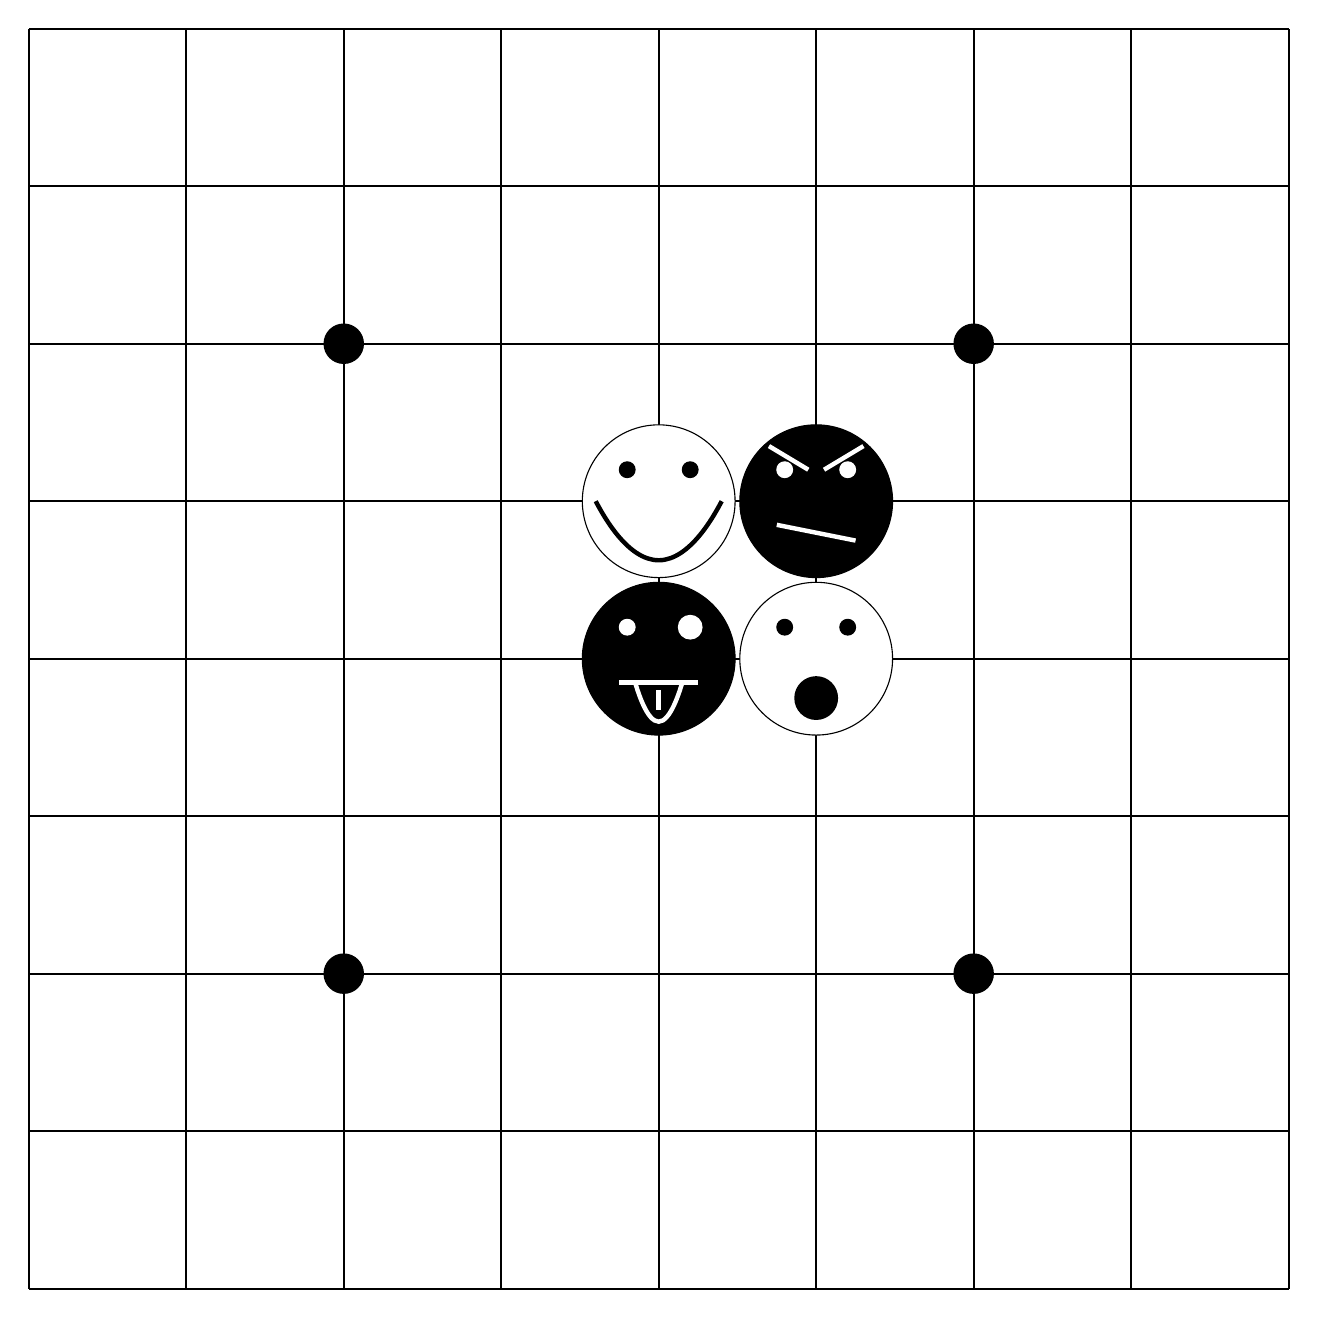
\begin{tikzpicture}

    \draw[thick] grid[step=2] (16,16);

    \draw[black,fill=black] (4,4) circle[radius=0.25cm];
    \draw[black,fill=black] (12,4) circle[radius=0.25cm];
    \draw[black,fill=black] (4,12) circle[radius=0.25cm];
    \draw[black,fill=black] (12,12) circle[radius=0.25cm];
    \draw[black,fill=black] (8,8) circle[radius=0.25cm];

    % First black stone
    \draw[black,fill=black] (10,10) circle[radius=0.97cm];

    %% Eyes
    \draw[white,fill=white] (9.6,10.4) circle[radius=0.1cm];
    \draw[white,fill=white] (10.4,10.4) circle[radius=0.1cm];

    %% Mouth
    \draw[white,fill=white,ultra thick] (9.5, 9.7) -- (10.5, 9.5);

    %% Eyebrows

    \draw[white,fill=white, ultra thick] (9.9, 10.4) -- (9.4,10.7);
    \draw[white,fill=white, ultra thick] (10.1, 10.4) -- (10.6,10.7);
    

    % Second black stone
    \draw[black,fill=black] (8,8) circle[radius=0.97cm];

    %% Eyes
    \draw[white,fill=white] (7.6,8.4) circle[radius=0.1cm];
    \draw[white,fill=white] (8.4,8.4) circle[radius=0.15cm];

    %% Mouth
    \draw[white, fill=white,ultra thick] (7.5,7.7) -- (8.5,7.7);

    %% Tongue
    \draw[white, ultra thick] (7.7, 7.7) parabola[parabola height=-0.5cm] (8.3,7.7);
    \draw[white, ultra thick] (8, 7.35) -- (8, 7.6);
    
    % First white stone
    \draw[black,fill=white] (10,8) circle[radius=0.97cm];

    % Eyes
    \draw[black,fill=black] (9.6,8.4) circle[radius=0.1cm];
    \draw[black,fill=black] (10.4,8.4) circle[radius=0.1cm];

    % Mouth
   \draw[black,fill=black, ultra thick] (10,7.5) circle[radius=0.25cm];

   % Second white stone
   \draw[black,fill=white] (8,10) circle[radius=0.97cm];

   %% Eyes
   \draw[black,fill=black] (7.6,10.4) circle[radius=0.1cm];
   \draw[black,fill=black] (8.4,10.4) circle[radius=0.1cm];

   %% Mouth

   \draw[black, ultra thick] (7.2,10) parabola[parabola height=-0.75cm] (8.8,10);
   
  \end{tikzpicture}
\end{center}

\begin{enumerate}
\item Take turns with a friend.\\
  One is black, the other white.
\item You can draw only one stone in your turn.  
\item First one to capture wins.
\item Feel free to draw funny faces.
  
\begin{tikzpicture}[scale=0.3]
    % Second white stone
   \draw[black,fill=white] (8,10) circle[radius=0.97cm];

   %% Eyes
   \draw[black,fill=black] (7.6,10.4) circle[radius=0.1cm];
   \draw[black,fill=black] (8.4,10.4) circle[radius=0.1cm];

   %% Mouth

   \draw[black, ultra thick] (7.2,10) parabola[parabola height=-0.75cm] (8.8,10);
  \end{tikzpicture}
  
\begin{tikzpicture}[scale=0.3]
    % First black stone
    \draw[black,fill=black] (10,10) circle[radius=0.97cm];

    %% Eyes
    \draw[white,fill=white] (9.6,10.4) circle[radius=0.1cm];
    \draw[white,fill=white] (10.4,10.4) circle[radius=0.1cm];

    %% Mouth
    \draw[white,fill=white,ultra thick] (9.5, 9.7) -- (10.5, 9.5);

    %% Eyebrows

    \draw[white,fill=white, ultra thick] (9.9, 10.4) -- (9.4,10.7);
    \draw[white,fill=white, ultra thick] (10.1, 10.4) -- (10.6,10.7);
  \end{tikzpicture}
\end{enumerate}

\newpage

\begin{center}
  Count Territory

  \bigskip

  \cleargoban
  \largegoban
  \gobansize{9}
  \white{c1,c2,c3,c4,c5,b5,a5}
  %\gobansymbols{a1,b1,a2,b2,a3,b3,a4,b4}{1}
  \showgoban[a1,d6]

  \begin{tikzpicture}[overlay, remember picture]
    \draw (-1.2,1.4) node[font=\large,fill=white,opacity=0.8,circle,inner sep=0] {1};
    \draw (-0.4,1.4) node[font=\large,fill=white,opacity=0.8,circle,inner sep=0] {2};

    \draw (-1.2,2.2) node[font=\large,fill=white,opacity=0.8,circle,inner sep=0] {3};
    \draw (-0.4,2.2) node[font=\large,fill=white,opacity=0.8,circle,inner sep=0] {4};

    \draw (-1.2,3.0) node[font=\large,fill=white,opacity=0.8,circle,inner sep=0] {5};
    \draw (-0.4,3.0) node[font=\large,fill=white,opacity=0.8,circle,inner sep=0] {6};

    \draw (-1.2,3.8) node[font=\large,fill=white,opacity=0.8,circle,inner sep=0] {7};
    \draw (-0.4,3.8) node[font=\large,fill=white,opacity=0.8,circle,inner sep=0] {8};    
  \end{tikzpicture}

  White has \ul{8} points.

  \bigskip
  
  \noindent\rule{\textwidth}{2pt}

\bigskip

  Count Territory

  \bigskip

  \cleargoban
  \largegoban
  \gobansize{9}

  \black{h9,h8,h7,h6,h5,h4,j4}
  \showgoban[f2,j9]

  \begin{tikzpicture}[overlay, remember picture]
    \draw (1.2,3.7) node[font=\large,fill=white,opacity=0.8,circle,inner sep=0] {1};
    \draw (1.2,4.5) node[font=\large,fill=white,opacity=0.8,circle,inner sep=0] {2};
    \draw (1.2,5.3) node[font=\large,fill=white,opacity=0.8,circle,inner sep=0] {3};
    \draw (1.2,6.1) node[font=\large,fill=white,opacity=0.8,circle,inner sep=0] {4};
    \draw (1.2,6.9) node[font=\large,fill=white,opacity=0.8,circle,inner sep=0] {5};    
  \end{tikzpicture}

  Black has \ul{5} points.

  \newpage
  
  Count Territory

  \bigskip
  
\cleargoban  
%\white{#2}
%\black{#3}
\black{g7,g3,e5,d4,e6,e3,f7,f8,e2,f1,f2,e4,g9}
\white{c3,c7,d5,c4,d6,e7,e8,d2,e1,d1,d3,f9,e9}
\largegoban
\gobansize{9}
\showgoban[a1,i9]

  \begin{tikzpicture}[overlay, remember picture]
    \draw (-3.1,1.4) node[font=\large,fill=white,opacity=0.8,circle,inner sep=0] {1};
    \draw (-2.3,1.4) node[font=\large,fill=white,opacity=0.8,circle,inner sep=0] {2};
    \draw (-1.5,1.4) node[font=\large,fill=white,opacity=0.8,circle,inner sep=0] {3};

    \draw (-3.1,2.2) node[font=\large,fill=white,opacity=0.8,circle,inner sep=0] {4};
    \draw (-2.3,2.2) node[font=\large,fill=white,opacity=0.8,circle,inner sep=0] {5};
    \draw (-1.5,2.2) node[font=\large,fill=white,opacity=0.8,circle,inner sep=0] {6};

    \draw (-3.1,3.0) node[font=\large,fill=white,opacity=0.8,circle,inner sep=0] {7};
    \draw (-2.3,3.0) node[font=\large,fill=white,opacity=0.8,circle,inner sep=0] {8};

    \draw (-3.1,3.75) node[font=\large,fill=white,opacity=0.8,circle,inner sep=0] {9};
    \draw (-2.3,3.75) node[font=\large,fill=white,opacity=0.8,circle,inner sep=0] {10};    

    \draw (-3.1,4.5) node[font=\large,fill=white,opacity=0.8,circle,inner sep=0] {11};
    \draw (-2.3,4.5) node[font=\large,fill=white,opacity=0.8,circle,inner sep=0] {12};
    \draw (-1.5,4.5) node[font=\large,fill=white,opacity=0.8,circle,inner sep=0] {13};

    \draw (-3.1,5.35) node[font=\large,fill=white,opacity=0.8,circle,inner sep=0] {14};
    \draw (-2.3,5.35) node[font=\large,fill=white,opacity=0.8,circle,inner sep=0] {15};
    \draw (-1.5,5.35) node[font=\large,fill=white,opacity=0.8,circle,inner sep=0] {16};

    \draw (-3.1,6.1) node[font=\large,fill=white,opacity=0.8,circle,inner sep=0] {17};
    \draw (-2.3,6.1) node[font=\large,fill=white,opacity=0.8,circle,inner sep=0] {18};
    \draw (-0.75,6.1) node[font=\large,fill=white,opacity=0.8,circle,inner sep=0] {19};

    \draw (-3.1,6.85) node[font=\large,fill=white,opacity=0.8,circle,inner sep=0] {20};
    \draw (-2.3,6.85) node[font=\large,fill=white,opacity=0.8,circle,inner sep=0] {21};
    \draw (-1.5,6.85) node[font=\large,fill=white,opacity=0.8,circle,inner sep=0] {22};    
    \draw (-0.75,6.85) node[font=\large,fill=white,opacity=0.8,circle,inner sep=0] {23};

    \draw (-3.1,7.6) node[font=\large,fill=white,opacity=0.8,circle,inner sep=0] {24};
    \draw (-2.3,7.6) node[font=\large,fill=white,opacity=0.8,circle,inner sep=0] {25};
    \draw (-1.5,7.6) node[font=\large,fill=white,opacity=0.8,circle,inner sep=0] {26};    
    \draw (-0.75,7.6) node[font=\large,fill=white,opacity=0.8,circle,inner sep=0] {27};
  \end{tikzpicture}

  \begin{tikzpicture}[overlay, remember picture]
    \draw (1.4,2.45) node[font=\large,fill=white,opacity=0.8,circle,inner sep=0] {1};
    \draw (2.2,2.45) node[font=\large,fill=white,opacity=0.8,circle,inner sep=0] {2};
    \draw (3.0,2.45) node[font=\large,fill=white,opacity=0.8,circle,inner sep=0] {3};

    \draw (1.4,3.2) node[font=\large,fill=white,opacity=0.8,circle,inner sep=0] {4};
    \draw (2.2,3.2) node[font=\large,fill=white,opacity=0.8,circle,inner sep=0] {5};
    \draw (3.0,3.2) node[font=\large,fill=white,opacity=0.8,circle,inner sep=0] {6};

    \draw (0.7,4.0) node[font=\large,fill=white,opacity=0.8,circle,inner sep=0] {7};
    \draw (2.2,4.0) node[font=\large,fill=white,opacity=0.8,circle,inner sep=0] {8};
    \draw (3.0,4.0) node[font=\large,fill=white,opacity=0.8,circle,inner sep=0] {9};    

    \draw (0.7,4.75) node[font=\large,fill=white,opacity=0.8,circle,inner sep=0] {10};
    \draw (1.4,4.75) node[font=\large,fill=white,opacity=0.8,circle,inner sep=0] {11};        
    \draw (2.2,4.75) node[font=\large,fill=white,opacity=0.8,circle,inner sep=0] {12};
    \draw (3.0,4.75) node[font=\large,fill=white,opacity=0.8,circle,inner sep=0] {13};        

    \draw (0.7,5.5) node[font=\large,fill=white,opacity=0.8,circle,inner sep=0] {14};
    \draw (1.4,5.5) node[font=\large,fill=white,opacity=0.8,circle,inner sep=0] {15};        
    \draw (2.2,5.5) node[font=\large,fill=white,opacity=0.8,circle,inner sep=0] {16};
    \draw (3.0,5.5) node[font=\large,fill=white,opacity=0.8,circle,inner sep=0] {17};

    \draw (0.7,6.3) node[font=\large,fill=white,opacity=0.8,circle,inner sep=0] {18};
    \draw (1.4,6.3) node[font=\large,fill=white,opacity=0.8,circle,inner sep=0] {19};        
    \draw (2.2,6.3) node[font=\large,fill=white,opacity=0.8,circle,inner sep=0] {20};
    \draw (3.0,6.3) node[font=\large,fill=white,opacity=0.8,circle,inner sep=0] {21};

    \draw (2.2,7.05) node[font=\large,fill=white,opacity=0.8,circle,inner sep=0] {22};
    \draw (3.0,7.05) node[font=\large,fill=white,opacity=0.8,circle,inner sep=0] {23};

    \draw (1.4,7.8) node[font=\large,fill=white,opacity=0.8,circle,inner sep=0] {24};
    \draw (2.2,7.8) node[font=\large,fill=white,opacity=0.8,circle,inner sep=0] {25};
    \draw (3.0,7.8) node[font=\large,fill=white,opacity=0.8,circle,inner sep=0] {26};

    \draw (2.2,8.6) node[font=\large,fill=white,opacity=0.8,circle,inner sep=0] {27};
    \draw (3.0,8.6) node[font=\large,fill=white,opacity=0.8,circle,inner sep=0] {28};
  \end{tikzpicture}

\vspace{-2cm}
  
  {\Large White has \ul{27} points.\\
  Black has \ul{28} points.\\
  \ul{Black} wins.}
  
%% \begin{tikzpicture}[remember picture, overlay,shift={(-7.1,-2.35)}]
%%   \draw (4.3,3.1) node[font=\small] {a};
%%   \draw (5.05,3.1) node[font=\small] {b};
%%   \draw (5.8,3.1) node[font=\small] {c};
%%   \draw (6.55,3.1) node[font=\small] {d};
%%   \draw (7.3,3.1) node[font=\small] {e};
%%   \draw (8.05,3.1) node[font=\small] {f};
%%   \draw (8.8,3.1) node[font=\small] {g};
%%   \draw (9.6,3.1) node[font=\small] {h};
%%   \draw (10.35,3.1) node[font=\small] {j};
%%   %\draw (11.05,3.1) node[font=\small] {l};

%%   \draw (3.5,3.6) node[font=\small] {1};
%%   \draw (3.5,4.4) node[font=\small] {2};
%%   \draw (3.5,4.4 + 0.775) node[font=\small] {3};
%%   \draw (3.5,4.4 + 2*0.775) node[font=\small] {4};
%%   \draw (3.5,4.4 + 3*0.775) node[font=\small] {5};
%%   \draw (3.5,4.4 + 4*0.775) node[font=\small] {6};
%%   \draw (3.5,4.4 + 5*0.775) node[font=\small] {7};
%%   \draw (3.5,4.4 + 6*0.775) node[font=\small] {8};
%%   \draw (3.5,4.4 + 7*0.775) node[font=\small] {9};
%% \end{tikzpicture}

  \noindent\rule{\textwidth}{2pt}

\bigskip

  Count Territory

  \bigskip

  \vspace{1cm}
  
  \cleargoban

  \largegoban
  \gobansize{9}
  \black{d4,c7,f5,e7,d3,c5,b6,c2,d2,b1,f3,f4,e2,f8,g9,f9,f7,e6,f1,e1,a7,c1}
  \white{g7,g3,g5,c3,c4,b5,b4,b2,a3,a5,f2,g4,g2,g8,h9,j8,f6,g6,g1,a6,a2,a1}
  \showgoban[a1,i9]

  \begin{tikzpicture}[overlay, remember picture]
    \draw [decorate,
      decoration = {calligraphic brace,amplitude=20,mirror}, thick] (3.5,1.25) --  (3.5,6.25) node[midway,xshift=1.0cm,font=\Large] {7};
    \draw [decorate, decoration = {calligraphic brace,mirror,amplitude=5}, thick] (1.75, 1.0) -- (3.25,1.0) node[midway,yshift=-0.5cm,font=\Large] {2};

    \draw (-3.1,3.75) node[font=\large,fill=white,opacity=0.8,circle,inner sep=0] {1};
    \draw (-2.35,3.00) node[font=\large,fill=white,opacity=0.8,circle,inner sep=0] {2};

    \draw (2.2,6.75) node[font=\large,fill=white,opacity=0.8,circle,inner sep=0] {3};
    \draw (2.95,7.5) node[font=\large,fill=white,opacity=0.8,circle,inner sep=0] {4};


    \draw [decorate,
      decoration = {calligraphic brace,amplitude=10}, thick] (-3.25,8) --  (-3.5+5*0.75,8) node[midway,yshift=0.75cm,font=\Large] {5};
    \draw [decorate, decoration = {calligraphic brace,mirror,amplitude=5}, thick] (-3.4, 7.75) -- (-3.4,6.65) node[midway,xshift=-0.75cm,font=\Large] {2};

    \draw (-2.35,6.00) node[font=\large,fill=white,opacity=0.8,circle,inner sep=0] {1};
    \draw (-0.85,6.00) node[font=\large,fill=white,opacity=0.8,circle,inner sep=0] {2};

    \draw (-1.60,5.25) node[font=\large,fill=white,opacity=0.8,circle,inner sep=0] {3};
    \draw (-0.85,5.25) node[font=\large,fill=white,opacity=0.8,circle,inner sep=0] {4};

    \draw (-0.85,4.5) node[font=\large,fill=white,opacity=0.8,circle,inner sep=0] {5};
    \draw (-0.1,4.5) node[font=\large,fill=white,opacity=0.8,circle,inner sep=0] {6};

    \draw (-0.1,3.75) node[font=\large,fill=white,opacity=0.8,circle,inner sep=0] {7};

    \draw (-0.1,3.0) node[font=\large,fill=white,opacity=0.8,circle,inner sep=0] {8};

    \draw (-0.85,1.5) node[font=\large,fill=white,opacity=0.8,circle,inner sep=0] {9};
  \end{tikzpicture}

  {\Large White has \ul{$7$} $\times$ \ul{$2$} $+$ \ul{$4$} $=$ \ul{$7$} $+$ \ul{$7$} $+$ \ul{$4$} $=$ \ul{$18$} points.\\
  Black has \ul{$5$} $\times$ \ul{$2$} $+$ \ul{$9$} $=$ \ul{$5$} $+$ \ul{$5$} $+$ \ul{$9$} $=$ \ul{$19$} points.\\
  \ul{Black} wins.}
  
%% \begin{tikzpicture}[remember picture, overlay,shift={(-7.1,-2.35)}]
%%   \draw (4.3,3.1) node[font=\small] {a};
%%   \draw (5.05,3.1) node[font=\small] {b};
%%   \draw (5.8,3.1) node[font=\small] {c};
%%   \draw (6.55,3.1) node[font=\small] {d};
%%   \draw (7.3,3.1) node[font=\small] {e};
%%   \draw (8.05,3.1) node[font=\small] {f};
%%   \draw (8.8,3.1) node[font=\small] {g};
%%   \draw (9.6,3.1) node[font=\small] {h};
%%   \draw (10.35,3.1) node[font=\small] {j};
%%   %\draw (11.05,3.1) node[font=\small] {l};

%%   \draw (3.5,3.6) node[font=\small] {1};
%%   \draw (3.5,4.4) node[font=\small] {2};
%%   \draw (3.5,4.4 + 0.775) node[font=\small] {3};
%%   \draw (3.5,4.4 + 2*0.775) node[font=\small] {4};
%%   \draw (3.5,4.4 + 3*0.775) node[font=\small] {5};
%%   \draw (3.5,4.4 + 4*0.775) node[font=\small] {6};
%%   \draw (3.5,4.4 + 5*0.775) node[font=\small] {7};
%%   \draw (3.5,4.4 + 6*0.775) node[font=\small] {8};
%%   \draw (3.5,4.4 + 7*0.775) node[font=\small] {9};
%% \end{tikzpicture}


  Count Territory

  \bigskip

  \cleargoban
  \largegoban
  \gobansize{9}
  \black{e5,e3,e7,c5,b5,e2,g5,e8,h5,j5,f5,e1,e4,f9,e9,j6,g6,g4,a4,a5,c4,d3,f3,e6}
  \white{g3,g7,c3,b4,d2,b2,f8,h6,h8,h4,j3,f2,h2,f1,g9,f7,j7,h7,j4,a3,d1,b3,c1,f6}
  \showgoban[a1,i9]

  {\Large White has \smallrectangle $+$ \smallrectangle $+$ \smallrectangle $=$ \smallrectangle points.

    \vspace{0.5cm}
    
    Black has \smallrectangle $\times$ \smallrectangle $+$ \smallrectangle $=$ \smallrectangle points.\\

    \vspace{0.75cm}
    
    \rule{60pt}{2pt} wins.
    }

  
%%   \begin{tikzpicture}[remember picture, overlay,shift={(-7.1,-2.35)}]
%%   \draw (4.3,3.1) node[font=\small] {a};
%%   \draw (5.05,3.1) node[font=\small] {b};
%%   \draw (5.8,3.1) node[font=\small] {c};
%%   \draw (6.55,3.1) node[font=\small] {d};
%%   \draw (7.3,3.1) node[font=\small] {e};
%%   \draw (8.05,3.1) node[font=\small] {f};
%%   \draw (8.8,3.1) node[font=\small] {g};
%%   \draw (9.6,3.1) node[font=\small] {h};
%%   \draw (10.35,3.1) node[font=\small] {j};
%%   %\draw (11.05,3.1) node[font=\small] {l};

%%   \draw (3.5,3.6) node[font=\small] {1};
%%   \draw (3.5,4.4) node[font=\small] {2};
%%   \draw (3.5,4.4 + 0.775) node[font=\small] {3};
%%   \draw (3.5,4.4 + 2*0.775) node[font=\small] {4};
%%   \draw (3.5,4.4 + 3*0.775) node[font=\small] {5};
%%   \draw (3.5,4.4 + 4*0.775) node[font=\small] {6};
%%   \draw (3.5,4.4 + 5*0.775) node[font=\small] {7};
%%   \draw (3.5,4.4 + 6*0.775) node[font=\small] {8};
%%   \draw (3.5,4.4 + 7*0.775) node[font=\small] {9};
%% \end{tikzpicture}

  
\end{center}

\end{document}
